%% LyX 2.1.2 created this file.  For more info, see http://www.lyx.org/.
%% Do not edit unless you really know what you are doing.
\documentclass[doctor,xetex]{thuthesis}
\usepackage{graphicx}

\makeatletter
%%%%%%%%%%%%%%%%%%%%%%%%%%%%%% User specified LaTeX commands.
\usepackage{thutils}
\usepackage{nccbbb}
\newcommand{\thetitle}{人脸三维模型重建}
\newcommand{\theauthor}{梁鼎}
\newcommand{\eqname}{式}
% disable rubber spaces between paragraphs
\raggedbottom
% for parallel figure and table
\newcommand\figcaption{\def\@captype{figure}\caption}
\newcommand\tabcaption{\def\@captype{table}\caption}
% set width of rules in tables (better be added to ThuThesis)
\setlength{\heavyrulewidth}{1.5pt}
\setlength{\lightrulewidth}{1pt}
% adjust linespace in eqnarray
\setlength{\jot}{8bp}
\newcommand{\jota}{-0.3bp}
% allow page breaks within eqnarray
\allowdisplaybreaks
% bold italic in math
\def\mbi#1{\textbf{\emph{#1}}}
% set figure placement fractions
\renewcommand{\textfraction}{0.15}
\renewcommand{\topfraction}{0.85}
\renewcommand{\bottomfraction}{0.65}
\renewcommand{\floatpagefraction}{0.8}
% define where to break URLs
\def\UrlBreaks{\do\A\do\B\do\C\do\D\do\E\do\F\do\G\do\H\do\I\do\J\do\K\do\L\do\M\do\N\do\O\do\P\do\Q\do\R\do\S\do\T\do\U\do\V\do\W\do\X\do\Y\do\Z\do\[\do\\\do\]\do\^\do\_\do\`\do\a\do\b\do\c\do\d\do\e\do\f\do\g\do\h\do\i\do\j\do\k\do\l\do\m\do\n\do\o\do\p\do\q\do\r\do\s\do\t\do\u\do\v\do\w\do\x\do\y\do\z\do\0\do\1\do\2\do\3\do\4\do\5\do\6\do\7\do\8\do\9\do\.\do\@\do\\\do\/\do\!\do\_\do\|\do\;\do\>\do\]\do\)\do\,\do\?\do\'\do+\do\=\do\#}


\makeatother

\begin{document}

\chapter{人脸三维模型重建}

本章将着重阐述在已知相机参数条件下,利用多视角图片重建获得人脸三维面片模型。本章重点集中在\ref{sec:=0091CD=005EFA=004E09=007EF4=0070B9=004E91}节,该节详细介绍了通过双目匹配得到三维点云的方法,也是本工作的核心。\ref{sec:=0070B9=004E91=00878D=005408}节将介绍多个点云融合涉及的优化算法,生成mesh模型以及纹理贴图在\ref{sec:Mesh=006A21=00578B=00751F=006210=0053CA=007EB9=007406=008D34=0056FE}节简要介绍。




\section{重建三维点云\label{sec:=0091CD=005EFA=004E09=007EF4=0070B9=004E91}}


\subsection{算法流程}

\begin{figure}[tbph]
\begin{centering}
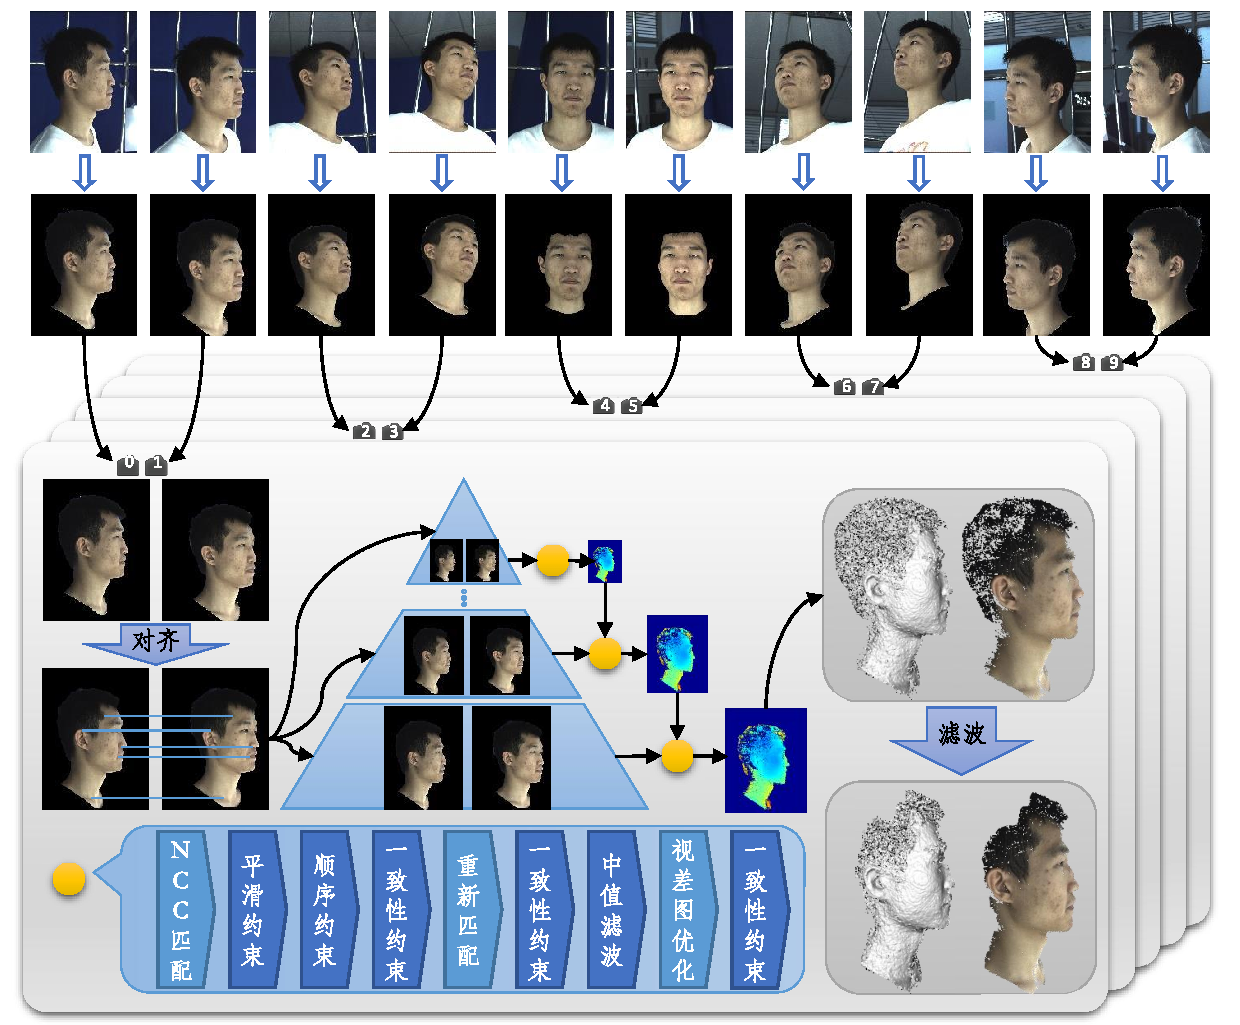
\includegraphics[width=1\columnwidth]{figures/chpt4/recons}
\par\end{centering}

\protect\caption{算法流程图}
\end{figure}



\subsection{算法模块}


\subsubsection{图片预处理}


\subsubsection{金字塔模型}


\subsubsection{图片对齐\label{sub:=0056FE=007247=005BF9=009F50}}


\subsubsection{NCC匹配计算视差图}


\subsubsection{约束限制}


\paragraph{顺序约束}


\paragraph{平滑约束}


\paragraph{一致性约束}


\subsubsection{重新匹配}


\subsubsection{中值滤波}


\subsubsection{视差图优化}


\subsubsection{从视差图到点云}


\section{点云融合\label{sec:=0070B9=004E91=00878D=005408}}


\section{Mesh模型生成及纹理贴图\label{sec:Mesh=006A21=00578B=00751F=006210=0053CA=007EB9=007406=008D34=0056FE}}


\subsection{泊松重建}


\subsection{表面平滑}


\subsection{纹理贴图}
\end{document}
